\chapter*{Introduction}
\label{cap:introduction}
\addcontentsline{toc}{chapter}{Introduction}

\chapterquote{Negar un hecho es lo más fácil del mundo. Mucha gente lo hace, pero el hecho sigue siendo un hecho.}{Isaac Asimov}
\section{¿Qué es APRS?}

APRS or Automatic Packet Reporting System (APRS) is a real-time digital communications system that allows the exchange of information between amateur radio stations.

In general, APRS is used for vehicle tracking, transmission of text messages, dissemination of weather information and communication in emergency situations, although due to the flexibility of the protocol it can be used in any other situation.

\begin{figure}[h!]
	\centering
	
\includegraphics[width=0.2\textwidth]{Imagenes/Chapter_1/APRS_logo.png}
	\caption{APRS logo.}
	\label{fig:aprs-logo}
\end{figure}

\section{Main APRS features}

APRS has several features that make it useful and versatile in the field of amateur radio communication, among which are the following:
\begin{itemize}
	\item \textbf{Working frequency:} APRS operates in the VHF band, specifically on the 144.80 MHz frequency in Europe, although other regions of the world use different frequencies as shown in the figure below. \Cref{fig:freq-map}.
	\item \textbf{Transmission mode:} APRS uses as a transmission mode individual packets that have to follow an established format, which greatly facilitates the adoption and integration of this technology.
	\item \textbf{Aprs retransmission policy:} In the APRS system, a packet of information is transmitted multiple times, gradually decreasing the emission frequency of these transmissions as time progresses. This method aims to maximize the packet reception rate.
\end{itemize}

\begin{figure}
	\centering
	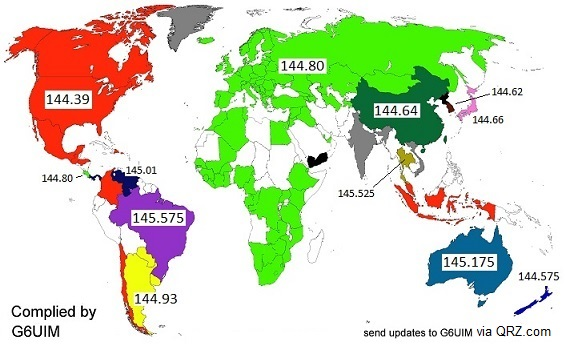
\includegraphics[width=0.5\textwidth]{Imagenes/Chapter_1/mapa_frecuencias_aprs.jpg}
	\caption{Aprs emission frequency around the globe.}
	\label{fig:freq-map}
\end{figure}


\section{Main APRS applications}

\begin{itemize}
	\item \textbf{GPS position reports:} APRS allows users to send their geographic location in the form of coordinates, obtained through GPS systems, which facilitates the tracking of vehicles or people in real time.

	\item \textbf{Weather data:} Weather stations often use APRS messages to report different data such as temperature, humidity or barometric pressure, including updated and useful information for various applications.

	\item \textbf{Internet integration:} Through the APRS-IS system, APRS messages are accessible over the Internet through different nodes, extending the reach and scope of this system.

	\item \textbf{Uso en Emergencias:} In emergency situations, APRS is a vital tool for broadcast communication and tracking of resources and personnel.
\end{itemize}

\section{History and Development of APRS}

The APRS system was born in the 1980s by Bob Bruninga, an engineer working at the U.S. Naval Academy. Bruninga created the first implementation of APRS on an Apple II computer in 1982 for the purpose of mapping Navy position reports on the high seas.\footnote{\url{http://www.aprs.org/APRS-docs/ARTICLES.TXT}} %\cite{einstein,latexcompanion,knuthwebsite}

The first real use of APRS was in 1984, when Bruninga developed a more advanced version on a VIC-20 to report the position and status of horses in an endurance race.

Over the next few years, Bruninga continued to refine the system, which he later dubbed the Connectionless Emergency Traffic System (CETS).

After a series of Federal Emergency Management Agency (FEMA) exercises using CETS, the system was moved to the IGM Pc. During the 1990s, CETS (now known as the Automatic Position Reporting System) continued to evolve.

As GPS technology became more widely available, the term ``Positioning'' was replaced by ``Package'' to better represent the broader capabilities of the system and emphasize its uses beyond mere position reporting.

\begin{figure}[h]
	\centering
	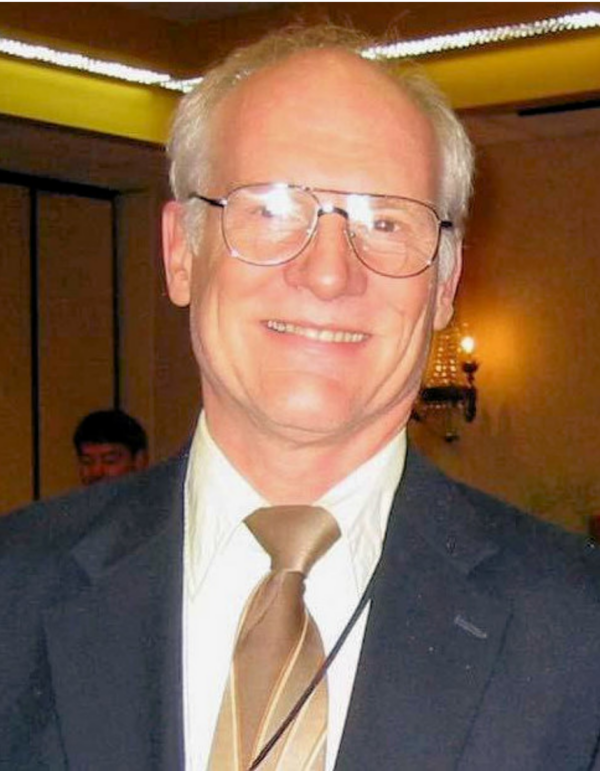
\includegraphics[width=0.15\textwidth]{Imagenes/Chapter_1/bob_bruninga.png}
	\caption{Bob Bruninga (creator of the APRS system).}
	\label{fig:bob-bruninga}
\end{figure}